\documentclass[prd,preprintnumbers,twocolumn,eqsecnum,floatfix,a4paper,nofootinbib,superscriptaddress]{revtex4}
\usepackage{color}
\usepackage{calc}
\usepackage{amsmath,amssymb,graphicx}
\usepackage{amssymb,amsmath}
\usepackage{bm}
\usepackage{microtype}
\usepackage{booktabs}
\usepackage{times}
\usepackage{subfigure}
\usepackage[varg]{txfonts}
\usepackage[colorlinks, pdfborder={0 0 0}]{hyperref}
\usepackage[utf8]{inputenc}
\definecolor{LinkColor}{rgb}{0.75, 0, 0}
\definecolor{CiteColor}{rgb}{0, 0.5, 0.5}
\definecolor{UrlColor}{rgb}{0, 0, 0.75}
\hypersetup{linkcolor=LinkColor}
\hypersetup{citecolor=CiteColor}
\hypersetup{urlcolor=UrlColor}
\maxdeadcycles=1000
\allowdisplaybreaks
\textwidth 7 in
\hoffset -0.1in
\textheight 10in
\DeclareFontFamily{OT1}{pzc}{}
\DeclareFontShape{OT1}{pzc}{m}{it}{<-> s * [1.10] pzcmi7t}{}
\DeclareMathAlphabet{\mathpzc}{OT1}{pzc}{m}{it}
\newcommand{\red}[1]{\textcolor{red}{#1}}
\newcommand{\comment}[1]{\textcolor{blue}{\textit{#1}}}
\newcommand{\ajith}[1]{\textcolor{red}{\textit{Ajith:#1}}}
\newcommand{\checkthis}{\textcolor{magenta}{(CHECKTHIS)}}
\newcommand{\vijay}[1]{\textcolor{cyan}{Vijay: #1}}
\newcommand{\io}{\iota}
\newcommand{\p}{\phi}
\newcommand{\vp}{\varphi}

\newcommand{\h}{\mathpzc{h}}
\newcommand{\Hhat}{\hat{\mathpzc{H}}}
\newcommand{\B}{\mathpzc{B}}
\newcommand{\hlm}{\mathpzc{h}_{\ell m}}
\newcommand{\xilm}{\xi_{\ell m}}
\newcommand{\Ylm}{{Y}^{-2}_{\ell m}}
\newcommand{\Y}{{Y}^{-2}}
\newcommand{\hc}{h_\times}
\newcommand{\hp}{h_+}
\newcommand{\Fc}{F_\times}
\newcommand{\Fp}{F_+}
\newcommand{\Mf}{M_f}
\newcommand{\cA}{\mathpzc{A}}
\newcommand{\lm}{_{\ell m}}
\newcommand{\deff}{d_\mathrm{eff}}
\newcommand{\rmi}{\mathrm{i}}
\newcommand{\blambda}{\bm{\lambda}}
\newcommand{\btheta}{\bm{\theta}}
\newcommand{\Mo}{M_{\odot}}
\newcommand{\FFe}{\mathrm{FF}_\mathrm{eff}}
\newcommand{\FF}{\mathrm{FF}}
\newcommand{\e}{\mathrm{e}}
\newcommand{\rhoopt}{\rho_\mathrm{opt}}
\newcommand{\rhosubopt}{\rho_\mathrm{subopt}}
\newcommand{\fqnm}{f}
\newcommand{\sigmaqnm}{\sigma}
\newcommand{\n}{\mathbf{n}}
\newcommand{\bxi}{\bm{\xi}}
\newcommand*{\skymapscale}{0.5}
\newcommand*{\paramestscale}{0.455}

\begin{document}

\newcommand{\be}{\begin{equation}}
\newcommand{\ee}{\end{equation}}
\newcommand{\ber}{\begin{eqnarray}}
\newcommand{\eer}{\end{eqnarray}}
\def\bea{\begin{eqnarray}}
\def\eea{\end{eqnarray}}
\newcommand{\etal}{\emph{et al}}

\title{Testing the ``no-hair'' nature of binary black holes \\using the consistency of multipolar gravitational radiation}
\author{Tousif Islam}
\affiliation{International Centre for Theoretical Sciences, Tata Institute of Fundamental Research, Bangalore 560012, India}
\author{Ajit Kumar Mehta}
\affiliation{International Centre for Theoretical Sciences, Tata Institute of Fundamental Research, Bangalore 560012, India}
\author{Abhirup Ghosh}
\affiliation{Max Planck Institute for Gravitational Physics (Albert Einstein Institute), D-14476 Potsdam-Golm, Germany}
\affiliation{International Centre for Theoretical Sciences, Tata Institute of Fundamental Research, Bangalore 560012, India}
\author{Vijay Varma}
\affiliation{Theoretical Astrophysics, 350-17, California Institute of Technology, Pasadena, CA 91125, USA}
\author{Parameswaran~Ajith}
\affiliation{International Centre for Theoretical Sciences, Tata Institute of Fundamental Research, Bangalore 560012, India}
\affiliation{Canadian Institute for Advanced Research, CIFAR Azrieli Global Scholar, MaRS Centre, West Tower, 661 University Ave., Suite 505, Toronto, ON M5G 1M1, Canada}
\author{B.~S.~Sathyaprakash}
\affiliation{Department of Physics and Department of Astronomy and Astrophysics, The Pennsylvania State University, University Park, PA 16802, USA}
\affiliation{School of Physics and Astronomy, Cardiff University, Cardiff, CF24 3AA, UK}


\begin{abstract}
\end{abstract}
\preprint{}
\maketitle
%%%%%%%%%%%%%%%%%%%%%%%%%%%%%%%%%%%%%%%%%%%%%%%%%%%%%%%%%%%%%%%%%%%%%%%%%%%%%%%%%%%%%%%%%%%%%%%%%%%%%%%%%%%%%%%%%%%%%%%%%%%%%%%%%%%%%%%%%%%%%%%`
\section{Introduction}

%%%%%%%%%%%%%%%%%%%%%%%%%%%%%%%%%%%%%%%%%%%%%%%%%%%%%%%%%%%%%%%%%%%%%%%%%%%%%%%%%%%%%%%%%%%%%%%%%%%%%%%%%%%%%%%%%%%%%%%%%%%%%%%%%%%%%%%%%%%%%%%`

\section{Testing the consistency of different multipoles of the radiation}

Recent gravitational-wave observations of colaescing compact binaries by LIGO and Virgo have provided a unique testbed for gravity. Due to their high compactness, the black holes and neutron stars in coalescing binaries move with speeds close to the speed of light before they collide with each other 

\ajith{I am happy to take a first stab at this, unless Sathya wants to take this up}

\subsection{Formulation of the test}

Gravitational wave radiation from by a binary black hole in GR consistst of two polarization states  $h_+(t)$ and $h_\times(t)$, which can be expressed as a complex time series $\h(t) := h_+(t) - i \, h_\times(t)$. The radiation can be written as a superposition of various spherical harmonic modes ${\h}_{\ell m}(t; \blambda)$ as~\cite{NewmanPenrose}:
\begin{equation} 
\h(t; \n, \blambda)= \frac{1}{d_L} \sum _{\ell=2}^{\infty} \sum _{m=-\ell}^{\ell} {\Ylm} (\n) \, {{\hlm}(t; {\blambda})}, 
\label{eq:spherical_harmonics}
\end{equation}
where $d_L$ is the luminosity distance to the binary, ${\Ylm}$ are spherical harmonics of weight $-2$ and $\n := \{\iota, \varphi_0\}$ define the direction of radiation in the source frame. The spherical harmonic modes, ${\h}_{lm}(t; \blambda)$, are purely functions of the \emph{intrinsic} parameters $\blambda$ of the system, such as the masses and spin angular momenta of the black holes. All the angular dependence of the radiation is captured by the spherical harmonic basis functions ${\Ylm}$. Thus, the multipolar structure (i.e., ${\h}_{lm}(t)$) of the waveform  is thus completely determined by the intrinsic parameters $\blambda$. 

 In GR, the leading order radiation is quadrupolar; i.e.,$\ell = 2, m = \pm 2$. The relative contribution of the higher modes depends on the total mass $M$, mass ratio $q$, spin angular momenta ${\mathbf S}_{1,2}$ and the inclination angle $\iota$.  Non-quadrupole modes becomes important when the black holes have  significantly unequal masses or when the spins are significantly misaligned with the orbital angular momentum. Furthermore, the strength of the higher mode amplitudes grows as the total mass and inclination angle increases. 

An interferometric GW detector observes a linear combination of the two polarizations $h_+ := \mathrm{Re}\,\h$ and $h_\times := - \mathrm{Im}\, \h$
\begin{equation}
h^I(t) = F^I_+(\theta, \phi, \psi) \, h_+(t-t_0^I) + F_{\times}^I(\theta, \phi, \psi)\, {h}_{\times}(t-t_0^I), 
\label{eq:det_response}
\end{equation}
where $F^I_+$ and $F^I_\times$ are the antenna pattern functions of the GW detector $I$, $t_0^I$ is the time of arrival of the signal at the detector, $(\theta, \phi)$ define the sky position and $\psi$ defines polarisation angle of the GW source, respectively. The signal is mixed with linear additive noise $n^I(t)$ in the detector, so that the observed data is $d^I(t) = h^I(t) + n^I(t)$. The noise can be modelled, to a good approximation, as a stationary Gaussian random process described by a power spectral density $S_n(f)$. By comparing theoretical templates of $h^I(t)$ with data $d$, we can infer the intrisic parameters of the binary as well as the extrinsic parameters describing the source position and orientation. 

As mentioned earlier, in GR the multipolar structure (i.e., ${\h}_{lm}(t)$) of the waveform from a binary black hole system is completely determined by its intrinsic parameters $\blambda$. Thus, if we estimate the parameters of the binary from different modes of the radiation, they have to be consistent with each other. However, if the true theory is different from GR or if the waveform is not emanated from a binary black hole system, this can, in general, change the multipolar structure of the waveform. Ref~\cite{Dhanpal:2018ufk} proposed a consistency test of the data with binary black holes in GR. The crux of the idea is to check the consistency of the intrinsic parameters estimated from different spherical harmonic modes of the waveform. Here we expand this idea and present different formulations of this test (i.e., different ways of introducing deviations from the GR multipolar waveform) and demonstrate these tests using simulated binary black hole observations. 

To model the GR waveforms, we employ the recent phenomenological inspiral-merger-ringdown waveform model proposed by~\cite{Mehta:2017jpq}, which provide accurate Fourier-domain models of three sub-dominant spherical harmonic modes ($(\ell = 2, m=\pm1)$, $(\ell = 3, m=\pm3)$, $(\ell = 4, m = \pm4)$) apart from the dominant $(\ell = 2, m = \pm2)$ mode of the expected GW signals from non-spinning BBHs. The other spherical harmonic modes neglected in this work only introduce an inaccuracy (mismatch) of less than 1\% in the waveforms~\cite{Mehta:2017jpq}. 
%We consider binaries with total mass $M := m_1 + m_2$ in the range $40 M_\odot$ -- 200 $M_\odot$ with mass ratio $q := m_2/m_1$ in the range 1/9 -- 1, with varying inclination angles $\iota=\{30^{\circ},45^{\circ},60^{\circ},80^{\circ},90^{\circ}\}$.

%\subsection{Parameterized tests of GR}
%\label{2b}
%In order to test GR, we extend the waveform model by incorporating additional deviation parameters.  We consider four independent ways to formulate efficient parameterized tests:

We introduce the following kinds of deviations in our GR waveform model: 

\paragraph{Formulation A:}
	Following ~\cite{dhanpal2018}, we generalize the GR waveform model Eq.~(\ref{eq:spherical_harmonics}) by allowing inconsistency between the intrinsic parameters determining the dominant mode and the higher order modes by introducing a set of deviation $\Delta \blambda := \{\Delta M_c, \Delta q\}$ in the higher modes (details in Section \ref{sec:simulationsa}):
	\begin{eqnarray}
	\h(t; \n, \blambda, \Delta \blambda) & = &  \frac{1}{d_L} \left[ ~ \sum_{m = \pm2} Y^{-2}_{2m} (\n) {\h}_{2m}(t, \blambda) \right. \nonumber \\ 
	& + & \left. \sum _{\text{H.O.M}} \Ylm (\n) \hlm(t, \blambda+\Delta \blambda), \right]
	\label{eq:test_1}
	\end{eqnarray}
where {H.O.M} indicates sum over higher order modes (all modes other than $\ell = 2, m = \pm 2$). 
	
\paragraph{Formulation B:}
	We modify the amplitudes of the higher modes and rewrite Eq.~(\ref{eq:spherical_harmonics}) as
	\begin{eqnarray}
	{\h}(t; \n, \blambda, c_{\ell m}) & = & \frac{1}{d_L} \left[ \sum_{m = \pm2} Y^{-2}_{2m} (\n) {\h}_{2m}(t, \blambda)  \right. \nonumber \\ 
	& + & \left. \sum _{\text{H.O.M}} (1+{c_{\ell m}}) \, \Ylm (\n) \hlm(t, \blambda), \right] 
	\label{eq:test_2}
	\end{eqnarray}
	where $c_{\ell m}$ is the deviation parameter and could be different for different higher order modes. We consident different combinations of ${c_{\ell m}}$ (details in Section \ref{sec:simulationsb}). 
	
% 	\item We include a deviation parameter $\Delta \blambda := \{\Delta M_c, \Delta q\}$ in the `cross' polarization of the GW radiation allowing a departure from GR (details in Section \ref{sec4a}):
% 	\begin{eqnarray} 
% 	\h(t; \blambda, \Delta \blambda) =  h_+(t; \blambda) - ih_\times(t; \blambda, \Delta \blambda),
% 	\label{eq:test_3}
% 	\end{eqnarray}
% 	
% 	\item We replace the two polarizations by 
% 	\begin{eqnarray} 
% 	\Hat{h_+}(f; \blambda)  \longrightarrow \Hat{h_+}(f; \blambda, \Delta \btheta) =h^{GR}_+ + i v f h^{GR}_{\times} 
% 	\label{eq:test_4a}
% 	\end{eqnarray}
% 	\begin{eqnarray}
% \Hat{h_\times}(f; \blambda) \longrightarrow \Hat{h_\times}(f; \blambda, \Delta \btheta) =h^{GR}_\times - i v f h^{GR}_{+}
% 	\label{eq:test_4b}
% 	\end{eqnarray}
% 	where $\btheta=\{v\}$ introduces deformation to the GR waveform and is exactly zero in GR (details in Section \ref{sec4b}).
		


\subsection{Bayesian analysis}

% The gravitational wave strain observed by a detector can be expressed as
% \begin{equation}
% h(t) = F_+(\theta, \phi, \psi) \, h_+(t-t_0) + F_{\times}(\theta, \phi, \psi)\, {h}_{\times}(t-t_0), 
% \label{eq:det_response}
% \end{equation}
% where the antenna pattern functions of the GW detector $F_+$ and $F_\times$  depend only on the source location $(\theta, \phi)$ and polarization angle of the gravitational wave $\psi$.  The time of arrival of the signal at the detector is denoted by $t_0$. For coalescing BBH systems in quasi-circular orbits, the measured strain $h(t)$ is therefore described by a set of \emph{intrinsic} parameters $\blambda = \{M_c, q\}$ and \emph{extrinsic} parameters  $\btheta := \{t_0, \iota, \varphi_0, d_L, \theta, \phi, \psi\}$ in GR. In addition to the parameters that describe signals in GR, we introduce a set of intrinsic parameters $\Delta \blambda$ and extrinsic parameters $\Delta \btheta$  which captures any possible departure from GR.  (The nature of these deviation parameters is outlined in Section \ref{2b} while details are given in Section \ref{sec:simulations} and Section \ref{sec4}). The deviation parameters $\Delta \blambda$ ($\Delta \btheta$) describes difference between the intrinsic (extrinsic) parameters used to generate the dominant and sub-dominant modes or the `plus' and `cross' polarizations. The combined set of parameters in our waveform model thus becomes $\bxi = \{\blambda, \btheta, \Delta \blambda\}$ (first \& third tests in Section \ref{2b}) or $\bxi = \{\blambda, \btheta, \Delta \btheta\}$ (second \& fourth tests in Section \ref{2b}). 

We assume that the data $d^I(t) = n^I(t) + h^I(t;\bxi)$ in each detector consist of noise and a GW signal $h^I(t; \bxi)$, described by a set of parameters $\bxi$. The noise is further assumed to be described by a stationary Gaussian random process of zero mean and a power spectral density $S_n(f)$. Given data $d(t)$ and the model $h^I(t; \bxi)$, the posterior probability distribution of the set of parameters ${\bxi}$ is given by the Bayes theorem: 
\begin{equation}
P({\bxi} \, | \, d, H) = \frac{P({\bxi} \, | \, H) \, P (d \, | \, {\bxi}, H)}{P(d \, | \, H)}.
\label{eq:Bayes_theorem}
\end{equation} 
Prior $P({\bxi} \, | \, H)$ denotes the probability of the parameters given the Hypothesis.  The likelihood $P (d \, | \, {\bxi}, H)$ gives the probability of observing data $d(t)$ given the model parameter $\bxi$; and $P(d \, | \, H)$ is a normalization constant, called the \emph{evidence} or the \emph{marginal likelihood}, expressed as:
 \begin{equation}
 P(d \, | \, H)=\int p(d|\bxi, H)p(\bxi | H)d\bxi.
 \label{eq:evidence}
 \end{equation}
For stationary Gaussian noise with power spectral density $S_n(f)$, the likelihood is written as:
\begin{equation}
P (d \, | \, {\bxi}, H) = \text{exp}\left[ -\frac{1}{2}\int_{f_\mathrm{low}}^{f_\mathrm{high}} \frac{|\tilde{d}(f) - \tilde{h}(f;{\bxi}, H)|^2}{S_n(f)}df\right],
\end{equation}
where $\tilde{d}(f)$ and $\tilde{h}(f)$ are the Fourier transforms of $d(t)$ and $h(t)$, respectively. The sensitivity bandwidth of the detector defines the limits of the integration $f_\mathrm{low}$ and $f_\mathrm{high}$. \ajith{Probably we could slightly expand this section by properly writing the likelihood in terms of inner products and so on. Abhirup, would you like to take this up?}

In this work, we consider a network of three global detectors consists of two Advanced LIGO detectors, at Hanford (H) and Livingston (L), and the Virgo detector (V) at Pisa. Advanced LIGO is considered to be in its ``high-power, zero-detuning'' configuration~\cite{aLIGOZeroDetHighPower} whereas Virgo is assumed to have its design-sensitivity. Assuming that the noise is uncorrelated in each detector, the network likelihood for data obtained from three detectors can thus be written as the product of the likelihoods in each detector
\begin{equation}
P (d \, | \, {\bxi}, H, S_n(f)) = \prod_{I \epsilon {H,L,V}} P (d^{I} \, | \, {\bxi}, H, S_{n_{i}}(f)).
\end{equation}

Using the Bayesian framework described above, we estimate $\bxi$ by stochastically sampling over the entire parameter space of interest. We use python-based affine-invariant ensemble sampler \texttt{emcee}~\cite{foreman2013emcee} for Markov chain Monte Carlo (MCMC) proposed by \cite{goodman2010ensemble} to obtain the posterior distribution $P(\bxi \, | \, d, H)$ of the full parameter set. Posterior distributions of particular parameters of interest, for example,  the set of parameters ${\Delta \blambda}$ or $c_{\ell m}$, describing deviation from the GR prediction of a BBH signal, are computed  by marginalizing the posterior over all other parameters $\{\blambda, \btheta\}$. If the data is consistent with a BBH signal in GR, we expect $P(\Delta \blambda \, | \, d, H)$ (or $P(\Delta c_{\ell m} \, | \, d, H)$) to be consistent with zero. 

Using simulated GR events, we compute the marginalized posterior distribution of the deviation parameters  ${\Delta \blambda}$ or $c_{\ell m}$. In order to compute the constraints on these parameters, we calculate the 90\% probability interval. Parameters which are recovered with greatest precision from the simulated GR signal will result smaller values for the credible interval and therefore would give more stringent test of GR with actual observation.

We assume the chirp mass $M_c \in [1,200] M_\odot$ and mass ratio $q \in [0.05,1.0]$ of BBH to have uniform distribution. The prior density function on the location of the source is  taken  to  be  isotropically  distributed  on  the  sphere of  the  sky,  with $P({dL} \, | \, H)=d_{L}^{2}$ with $d_L \in [1,10000]$ Mpc. Furthermore, we use an  isotropic  prior  on  the  orientation  of  the  binary: $P({\iota,\varphi_0,\psi} \, | \, H)=\sin\iota$ with $\iota \in [0,\pi]$, $\varphi \in [0,2\pi]$ and $\psi \in [0,\pi]$. For all other parameters in $\bxi$, we use uniform priors.

%%%%%%%%%%%%%%%%%%%%%%%%%%%%%%%%%%%%%%%%%%%%%%%%%%%%%%%%%%%%%%%%%%%%%%%%%%%%%%%%%%%%%%%%%%
\begin{figure}[tb] \begin{center}
		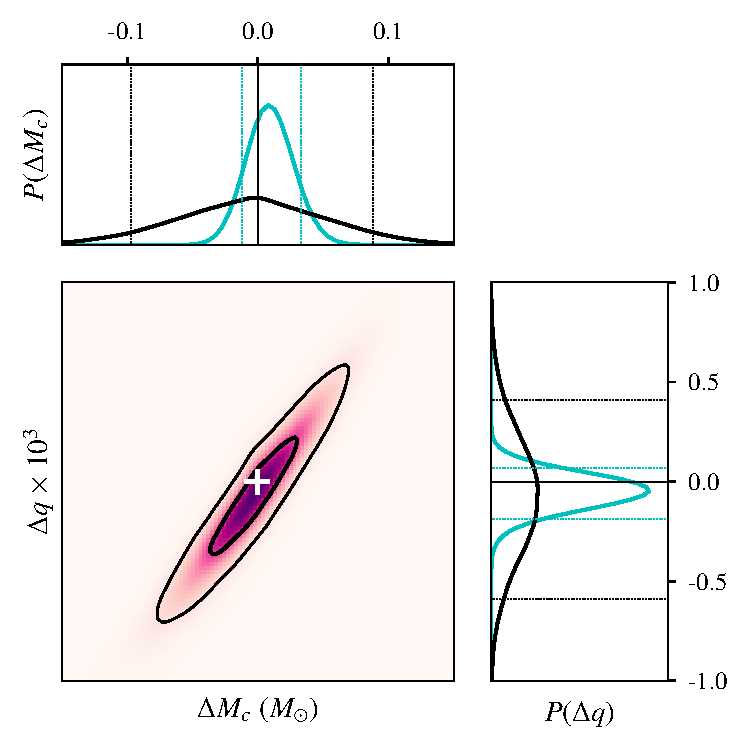
\includegraphics[width=3.4in]{figs/hm_mcq_GR.pdf}
		\caption{\emph{Middle panel}: the thick (thin) contours show the 50\% (90\%) credible regions in the joint posteriors of two parameters $\Delta M_c$ and $\Delta q$ that describe deviations in the estimated parameters using the quadrupole and non-quadrupole modes, estimated from a simulated GR signal [see Eq.~\eqref{eq:test_1} for the formulation]. \emph{Side panels}: Black histograms show the 1-dimesional posteriors in one deviation parameter (say, $\Delta M_c$) estimated from the joint posteriors, which is marginalized over the other (say, $\Delta q$). The cyan histograms show the 1-dimensional posteriors in $\Delta M_c$ and $\Delta q$ estimated from the data by introducing only one deviation parameter (say, $\Delta M_c$) at a time, keeping the other fixed (say, $\Delta q = 0$). The posteriors are fully consistent with the GR prediction of $\Delta M_c = \Delta q = 0$ (shown by a ``+'' sign in the center panel and by thin black lines in side panels). The dotted lines mark the 90\% credible regions. The simulated GR signal corresponds to a binary with total mass $M = {80}M_\odot$ and mass ratio $q = 1/9$ and an inclination angle $\iota = {60^\circ}$ observed by Advanced LIGO-Virgo detectors network with an optimal SNR of 25. SNR split in individual detectors are: 15 in LIGO-Hanford, 18.9 in LIGO-Livingston and 6.7 in Advanced Virgo.}
		\label{fig:posterior_BBH_GR_inj}
\end{center} \end{figure}
%%%%%%%%%%%%%%%%%%%%%%%%%%%%%%%%%%%%%%%%%%%%%%%%%%%%%%%%%%%%%%%%%%%%%%%%%%%%%%%%%%%%%%%%%%

%%%%%%%%%%%%%%%%%%%%%%%%%%%%%%%%%%%%%%%%%%%%%%%%%%%%%%%%%%%%%%%%%%%%%%%%%%%%%%%%%%%%%%%%%%
\begin{figure}[tb] \begin{center}
		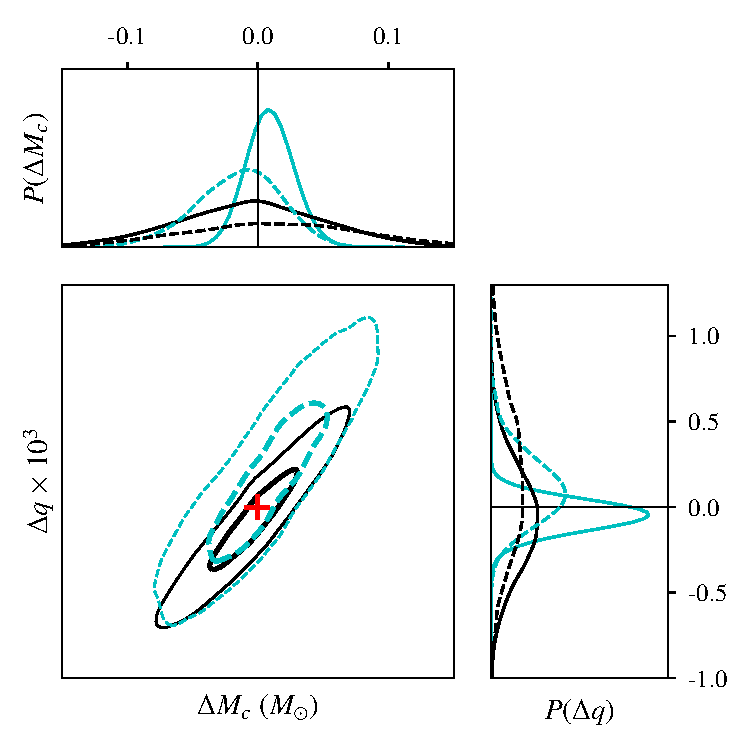
\includegraphics[width=3.4in]{figs/hm_mcq_1det_3det_compare_GR.pdf}
		\caption{Same as Fig.~\ref{fig:posterior_BBH_GR_inj} except that the dashed traces show the posteriors estimated using a single Advanced LIGO detector with SNR of 25. It can be seen that, as expected, posteriors from the three detector observation are tighter.}
		\label{fig:hm_mcq_compare-1det_3det_GR_inj}
	\end{center} \end{figure}
%%%%%%%%%%%%%%%%%%%%%%%%%%%%%%%%%%%%%%%%%%%%%%%%%%%%%%%%%%%%%%%%%%%%%%%%%%%%%%%%%%%%%%%%%%

%%%%%%%%%%%%%%%%%%%%%%%%%%%%%%%%%%%%%%%%%%%%%%%%%%%%%%%%%%%%%%%%%%%%%%%%%%%%%%%%%%%%%%%%%%
 \begin{figure}[tbh]
 	\begin{center}
 		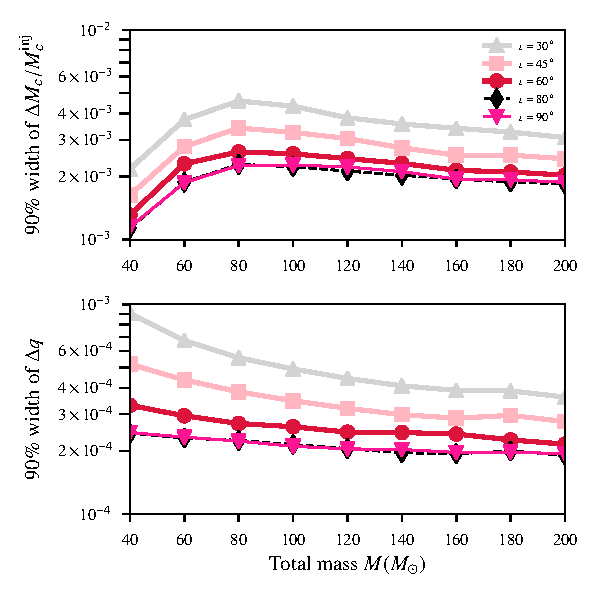
\includegraphics[scale=0.8]{figs/hm_9dim_dmcbymcinj_dq_diff_M.pdf}
 	\end{center} 
 	\caption{The figure shows the width of the 90$\%$ credible regions of the deviation parameters $\Delta M_c$ and $\Delta q$ for binaries with different total mass (horizontal axis) and inclination angles $\iota$ (legends). All binaries have an asymmetric mass ratio $q=1/9$.}
 	\label{fig:delmc_delq_varyingM}
 \end{figure}
 
 \begin{figure}[tbh]
 	\begin{center}
 		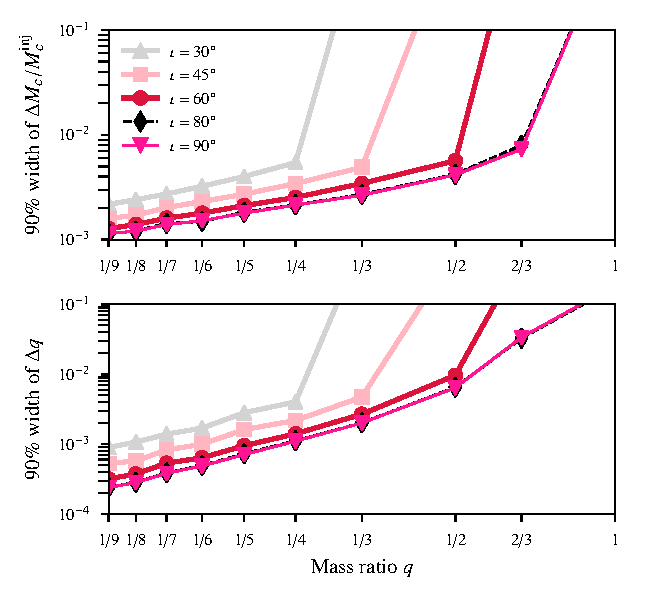
\includegraphics[scale=0.8]{figs/hm_9dim_dmcbymcinj_dq_diff_q.pdf}
 	\end{center} 
 	\caption{Same as Fig.~\ref{fig:delmc_delq_varyingM}, except that the horizontal axis reports the mass ratio $q$. All binaries correspond to a total mass $40M_{\odot}$.}
 	\label{fig:delmc_delq_varyingq}
 \end{figure}
%%%%%%%%%%%%%%%%%%%%%%%%%%%%%%%%%%%%%%%%%%%%%%%%%%%%%%%%%%%%%%%%%%%%%%%%%%%%%%%%%%%%%%%%%%

%%%%%%%%%%%%%%%%%%%%%%%%%%%%%%%%%%%%%%%%%%%%%%%%%%%%%%%%%%%%%%%%%%%%%%%%%%%%%%%%%%%%%%%%%%%%%%%%%%%%%%%%%%%%%%%%%%%%%%%%%%%%%%%%%%%%%%%%%%%%%%%`
\section{Simulations and results}
\label{sec:simulations}

We now elaborate on the two formulations of the tests of GR presented in Section \ref{2b} and present results from simulated GR observations. Our strategy, as described earlier, is to introduce extra parameters in the higher order modes of radiation --- parameters describing inconsistency between different modes --- and to constrain them using a Bayesian framework. 

\subsection{Formulation A:}
\label{sec:formulationA}
The first test we consider the formulation proposed in Eq.~\eqref{eq:test_1}. This follows the outline presented in ~\cite{dhanpal2018} to check for the consistency of intrinsic parameters $\blambda := \{M_c, q\}$ estimated from the dominant mode and the higher order modes. According to this, we would estimate the chirp mass and asymmetric mas ratio of the BBH from the leading quadrapolar mode of the observed signal. Independently, we would estimate them from the higher order modes. In GR, these two estimates of $M_c$ and $q$ should match and hence we expect the posterior distribution of $\Delta \blambda $ to be consistent with zero. While ~\cite{dhanpal2018} focuses on one performing this test with only one Advanced LIGO detector, we study the performance of this test in the case of the three detector Advanced LIGO-Virgo network. 

We consider two different ways to perform the test. First, we introduce \emph{one} deviation parameter at a time. That is, $\Delta\blambda = {\Delta M_c}$ or $\Delta\blambda = {\Delta q}$. We then consider introducing a concurrent deviation in \emph{two} parameters $\Delta \blambda = \{\Delta M_c, \Delta q\}$. In Fig.~\ref{fig:posterior_BBH_GR_inj}, we show the results of the tests performed with GR waveform by varying either one parameter or two parameters, for a binary with total mass $M = 80M_{\odot}$, mass ratio $q=1/9$, inclination angle $ {\iota}=60^{\circ} $ producing a network signal-to-noise ratio  (SNR)  of 25 (SNR in higher modes is $\sim 10$). SNRs in individual detectors are: 15 in Advanced LIGO-Hanford, 18.9 in Advanced LIGO-Livingston and 6.7 in Virgo. The posterior probability density for both the parameters $\Delta q$ and $\Delta M_c$ are consistent with zero as one expect in GR. Furthermore, the deviation parameters are found to be better constrained when only one deviation parameter is allowed to vary at a time (either $\Delta M_c$ or $\Delta q$). This suggests that a consistency test with only one deviation parameter in the higher modes would allow a more efficient test. In the subsequent analysis, we therefore focus on varying only one deviation parameter at a time. 

In Fig.~\ref{fig:hm_mcq_compare-1det_3det_GR_inj} we show that, as expected, the width of the posteriors of the deviation parameters become smaller (i.e., improved precision) when we perform the test with a network of three Advanced LIGO-Virgo detectors instead of using only one Advanced LIGO detector (for the same SNR). However, for a fixed SNR, the improvements in the precision is small (facor of $\sim ~\red{X}$), due to the fact that the improved information (e.g., sky localization) is not highly correlated with the intrinsic parameters $M_c, q$ nor the deviation parameters $\Delta M_c, q$. %A key difference between the one detector analysis in ~\cite{dhanpal2018} and the three detector analysis of this paper is that we now have three different times of arrival $\{ t_{0,H}, t_{0,L}, t_{0,V}\}$, compared to one in earlier case, that need to be sampled over. We instead choose to sample only the time of arrival of the signal at the center of earth and then compute $\{ t_{0,H}, t_{0,L}, t_{0,V}\}$ by adding a constant time delay between the geo-center and the respective detectors. 
\ajith{What exactly are the parameters that are sampled? $t_0$ and $\theta$, $\phi$?}

 Figures~\ref{fig:delmc_delq_varyingM} and \ref{fig:delmc_delq_varyingq} show the 90\% credible intervals of the posteriors of the deviation parameters for binaries with varying masses, mass ratios and inclination angles, estimated using the three detector network. In all cases, we set the network SNR to be {25}. Note that only one deviation parameter ($\Delta M_c$ or $\Delta q$) is varied at a time.  We find that binaries with large mass ratios ($q < 1/ 2$) and inclination angles ($\iota > 60 ^\circ $) will allow precision tests of the GR predictions, reaching statistical uncertainties of $< 10^{-3}$ for $\Delta q$ and $< 10^{-2}$ for the dimensionless deviation parameter $\Delta M_c/M_c$. Our results are found to be consistent with the one detector analysis done in ~\cite{dhanpal2018}. We, however, notice that the 90\% interval for both the deviation parameters, in three detector analysis, decreases slightly (i.e., precision improved) as compared to the one detector case.
 
\subsection{Formulation B}
\label{sec:formulationB}

% %%%%%%%%%%%%%%%%%%%%%%%%%%%%%%%%%%%%%%%%%%%%%%%%%%%%%%%%%%%%%%%%%%%%%%%%%%%%%%%%%%%%%%%%%%
%  \begin{figure}[tbh]
%  	\begin{center}
%  		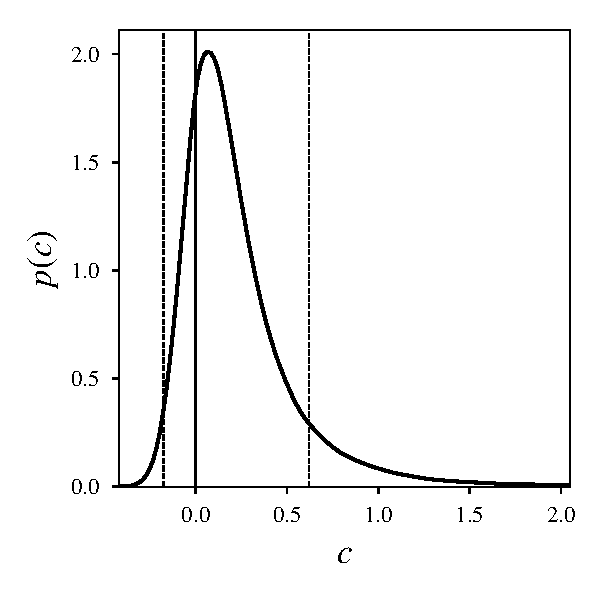
\includegraphics[scale=0.63]{figs/hist_c1_M_80_q_9_snr_25.pdf}
%  	\end{center} 
%  	\caption{The figure shows the posterior probability distribution of the deviation parameter $c$ estimated from the same simulated GR observation in Fig.~\ref{fig:posterior_BBH_GR_inj} (version 1 of the test described in Sec.~\ref{sec:formulationB}). Thin black lines shows the expected value in GR. The dotted lines mark the 90\% credible regions. \ajith{The difference between dashed and dotted lines not clear. Pl make the black vertical line solid. Also pl change the variable name from $c_1$ to $c$ in the plot}}
%  	\label{fig:c1_hist}
%  \end{figure}
% %%%%%%%%%%%%%%%%%%%%%%%%%%%%%%%%%%%%%%%%%%%%%%%%%%%%%%%%%%%%%%%%%%%%%%%%%%%%%%%%%%%%%%%%%%

%%%%%%%%%%%%%%%%%%%%%%%%%%%%%%%%%%%%%%%%%%%%%%%%%%%%%%%%%%%%%%%%%%%%%%%%%%%%%%%%%%%%%%%%%%
\begin{figure*}[tbh]
	\begin{center}
 		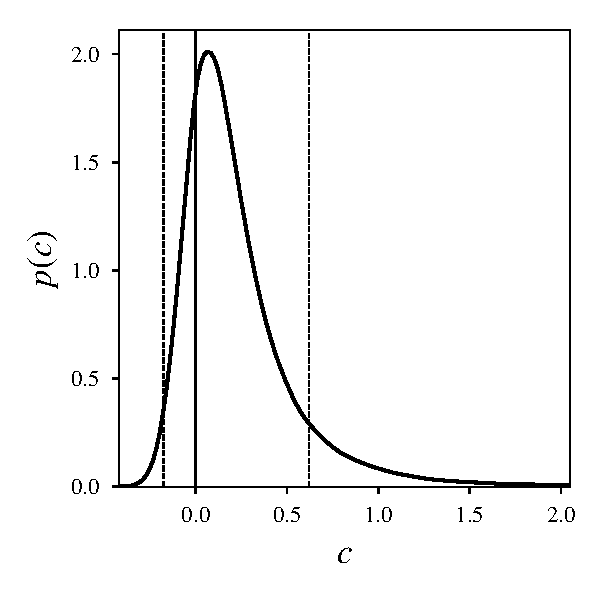
\includegraphics[height=2.1in]{figs/hist_c1_M_80_q_9_snr_25.pdf}
		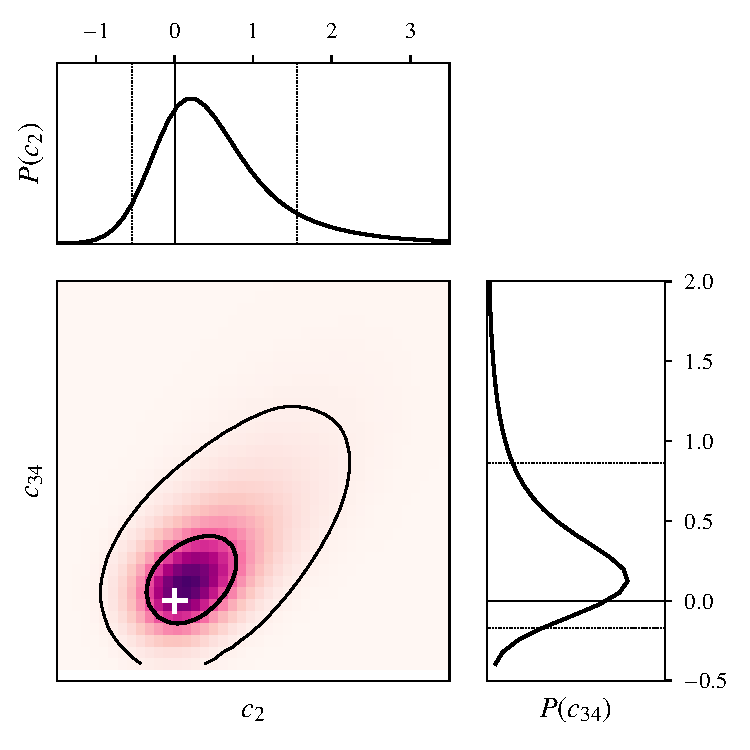
\includegraphics[height=2.4in]{figs/c2_c34_M_80_q_9_SNR_25.pdf}
		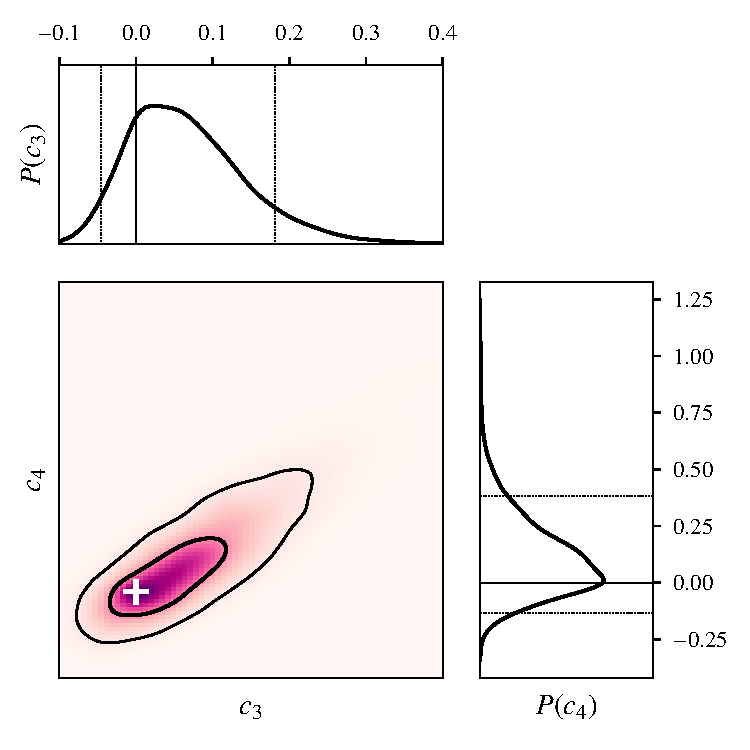
\includegraphics[height=2.4in]{figs/c3_c4_M_80_q_9_SNR_25.pdf}
	\end{center} 
 	\caption{\emph{Left:} The posterior probability distribution of the deviation parameter $c$ estimated from the same simulated GR observation in Fig.~\ref{fig:posterior_BBH_GR_inj} (version 1 of the test described in Sec.~\ref{sec:formulationB}). Thin black lines shows the expected value in GR. The dotted lines mark the 90\% credible regions. \emph{Middle:} Posteriors on $c_{21}$ and $c_{3344}$ from the same simulated observation (versoin 2 of the test). \emph{Right:} Posteriors on $c_{33}$ and $c_{44}$ from the same simulated observation (versoin 3 of the test). \ajith{In the left plot, the difference between dashed and dotted lines not clear. Pl make the black vertical line solid. Use black only in the left plot to make it consistent with the 1D posteriors from the middle and right plots. Also pl change the variable names to $c$, $c_{21}$, $c_{3344}$, etc.}}
	\label{fig:test2posts}
\end{figure*}
%%%%%%%%%%%%%%%%%%%%%%%%%%%%%%%%%%%%%%%%%%%%%%%%%%%%%%%%%%%%%%%%%%%%%%%%%%%%%%%%%%%%%%%%%%


%%%%%%%%%%%%%%%%%%%%%%%%%%%%%%%%%%%%%%%%%%%%%%%%%%%%%%%%%%%%%%%%%%%%%%%%%%%%%%%%%%%%%%%%%%
\begin{figure}[h]
	\begin{center}
		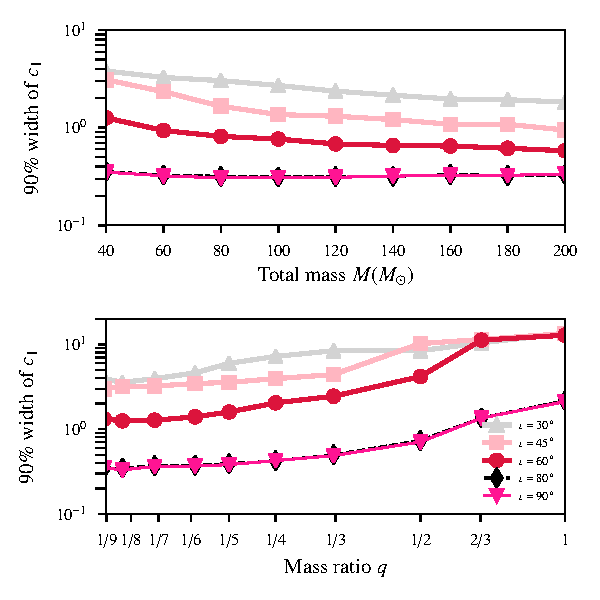
\includegraphics[scale=0.85]{figs/90_percent_CI_c1.pdf}
	\end{center} 
	\caption{The width of 90\% credible regions of the posteriors of $c$ for binaries with different total mass $M$ (upper panel) and mass ratio $q$ (lower panel) and inclination angle $\iota$ (legends). All binaries considered in the upper panel have a mass ratio $q=1/9$. Binaries considered in the lower panel have total mass of $40M_{\odot}$. All the simulated observations produce a network SNR of 25 in Advanced LIGO-Virgo network.}
	\label{fig:constraint_c}
\end{figure}
%%%%%%%%%%%%%%%%%%%%%%%%%%%%%%%%%%%%%%%%%%%%%%%%%%%%%%%%%%%%%%%%%%%%%%%%%%%%%%%%%%%%%%%%%%



Now we consider the formulation proposed in Eq.~\eqref{eq:test_2}, which involves introducing generic possible deviation parameters $c_{\ell m}$ in the amplitudes of the higher order modes. Indeed, the most general form of this test would treat all the $c_{\ell m}$ as free parameters. However, because of the correlation among these parameters and with some of the other parameters of the binary (such as the luminosity distance and inclination angle), this is likely to result in poor constraints on these parameters. Hence we consider different flavors of this test. 

\begin{enumerate}
\item We set $c := c_{21} = c_{33} = c_{44}$ and estimate the posteriors of $c$ along with all other binary parameters present in the GR waveform.  
\item We allow $c_{21}$ and $c_{3344} := c_{33} = c_{44} $ to vary and estimate the posteriors of $c_{21}$ and $c_{3344}$ along with all other binary parameters present in the GR waveform.  
\item We fix $c_{21} = 0$ and vary $c_{33}$ and $c_{44}$, thus estimating the posteriors of $c_{33}$ and $c_{44}$. 
\end{enumerate}

%  \begin{enumerate}
%  	\item We split the contributions from the dominant $(\ell = 2, m = \pm 2)$ mode of gravitational radiation, and the higher order modes in Eq.~(\ref{eq:spherical_harmonics}) and introduce a generic extrinsic deviation parameter $\Delta \btheta=\{c_1\}$ common for all the higher modes considered i.e. $(\ell = 2, m=\pm1)$, $(\ell = 3, m=\pm3)$, $(\ell = 4, m = \pm4)$.
%  	\begin{eqnarray}
%  	{\h}(t; n, \blambda, \Delta \btheta) & = & \frac{1}{d_L} \sum_{m = \pm2} Y^{-2}_{2m} (n) {\h}_{2m}(t, \blambda)  \nonumber \\ 
%  	& + & \frac{(1+{c_1})}{d_L} \sum _{\text{H.O.M}} \Ylm (n) \hlm(t, \blambda),
%  	\label{eq:test_c1}
%  	\end{eqnarray}
%  	where  H.O.M represents the higher order modes, and $\blambda$ be the intrinsic parameters. 	
%  
%  
%  	\item We then generalize the test by introducing a set of two different deviation parameter $\Delta \btheta=\{c_2, c_{34}\}$, where $c_2$ indicates the possible modification in the  $(\ell = 2, m=\pm1)$ mode and $c_{34}$ encodes a common deviation in $(\ell = 3, m=\pm3)$ and $(\ell = 4, m = \pm4)$ modes.
%  	\begin{eqnarray}
%  	{\h}(t; n, \blambda, \Delta \btheta) & = & \frac{1}{d_L} \sum_{m = \pm2} Y^{-2}_{2m} (n) {\h}_{2m}(t, \blambda)  \nonumber \\ 
%  	& + & \frac{(1+{c_2})}{d_L} \sum_{m = \pm1} Y^{-2}_{2m} (n) {\h}_{2m}(t, \blambda) \nonumber\\
%  	& + & \frac{(1+{c_{34}})}{d_L} \sum _{\text{33,44}} \Ylm (n) \hlm(t, \blambda),
%  	\label{eq:test_c2_c34}
%  	\end{eqnarray}
% 	
%  	\item In a futher generalization, we keep the amplitude of the quadrapole mode as well as the $(\ell = 2, m=\pm1)$ mode as predicted in GR and choose a set of two different deviation parameter $\Delta \btheta=\{c_3, c_{4}\}$ in the amplitudes of  $(\ell = 3, m=\pm3)$ mode and $(\ell = 4, m = \pm4)$ mode respectively.
%  	\begin{eqnarray}
%  	{\h}(t; n, \blambda, \Delta \btheta) & = & \frac{1}{d_L} \sum_{m = \pm2,\pm1} Y^{-2}_{2m} (n) {\h}_{2m}(t, \blambda)  \nonumber \\ 
%  	& + & \frac{(1+{c_3})}{d_L} \sum_{m = \pm3} Y^{-2}_{3m} (n) {\h}_{3m}(t, \blambda) \nonumber\\
%  	& + & \frac{(1+{c_{4}})}{d_L} \sum _{m=\pm4} Y^{-2}_{4m} (n) {\h}_{4m}(t, \blambda),
%  	\label{eq:test_c3_c4}
%  	\end{eqnarray}
%  \end{enumerate}

%The set of deviation parameters $\Delta \btheta=\{c_1\}$, $\Delta \btheta=\{c_2, c_{34}\}$ and $\Delta \btheta=\{c_3, c_{4}\}$ encodes possible departure from  GR. If there is no evidence of GR to be violated, all these deviation parameters would be consistent with zero. On the other hand, if GR is wrong, the posterior of these parameters $\Delta \btheta$, estimated from observations, would show a discrepancy with the expected value i.e. $\Delta \btheta=0$. 

In Fig.~\ref{fig:test2posts}, we show example posteriors of the deviation parameters obtained from a simulated binary black hole system (in GR) with  a total mass $M = 80M_{\odot}$, mass ratio $q=1/9$ and inclination angle $ {\iota}=60^{\circ} $, producing an SNR of 25 in the Advanced LIGO-Virgo network. The left plot shows the posterior of the deviation parameter $c$ (version 1 of the test), while the middle plot show the posteriors of $c_{21}$ and $c_{3344}$ (version 2 of the test) and the right panel shows the posteriors on $c_{33}$ and $c_{44}$  (versoin 3 of the test). We see that all the posterior distributions are consistent with zero. 

A more general version of these tests with amplitude correction in the higher modes would be to assume that the deviation parameters are complex in nature i.e. they have a magnitude as well as a phase component. To demonstrate such test, we replace the real amplitude correction $c$ (version 1 of the test) with a complex correction $\tilde{c} = |\tilde{c}| \, e^{\phi_c}$. Figure~\ref{fig:c1_complex} shows the posterior probability distribution of both the magnitude and phase of the deviation parameter $\tilde{c}$ from the same simulated GR event described in Fig.~\ref{fig:test2posts}. We find that though the absolute value of complex correction is well constrained, the phase remains uninformative. Hence for all the future tests we restrict to real valued deviation parameters. 

 %%%%%%%%%%%%%%%%%%%%%%%%%%%%%%%%%%%%%%%%%%%%%%%%%%%%
 \begin{figure}[tbh]
 	\begin{center}
 		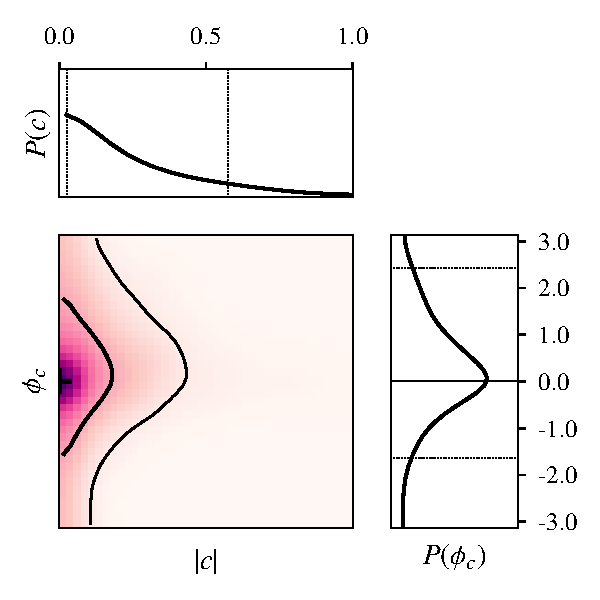
\includegraphics[scale=0.8]{figs/M_80_q_9_SNR_25_complex_c1.pdf}
 	\end{center} 
 	\caption{The figure shows the posterior probability distribution of the absolute value $|c_1|$and argument $\phi_c$ complex deviation parameter $\tilde{c_1}$ estimated from the simulated GR event. Details are same as in \ref{fig:posterior_BBH_GR_inj}.}
 	\label{fig:c1_complex}
 \end{figure}
 %%%%%%%%%%%%%%%%%%%%%%%%%%%%%%%%%%%%%%%%%%%%%%%%%%%%%
 


Figure \ref{fig:constraint_c} shows the width of the 90\% credible regions in the posterior of $c$  (version 1 of the test) as a function of the total mass and mass ratio of the binary (producing network SNR of 25 in all cases). Figure~\ref{fig:constraint_c21_c3344} shows the the width of the 90\% credible regions in the posteriors of $c_{21}$ and  $c_{3344}$  (version 2 of the test) while Fig.~\ref{fig:constraint_c33_c44} shows the same for $c_{33}$ and  $c_{44}$  (version 3 of the test). 

%%%%%%%%%%%%%%%%%%%%%%%%%%%%%%%%%%%%%%%%%%%%%%%%%%%%%
\begin{figure*}[tbh]
	\begin{center}
		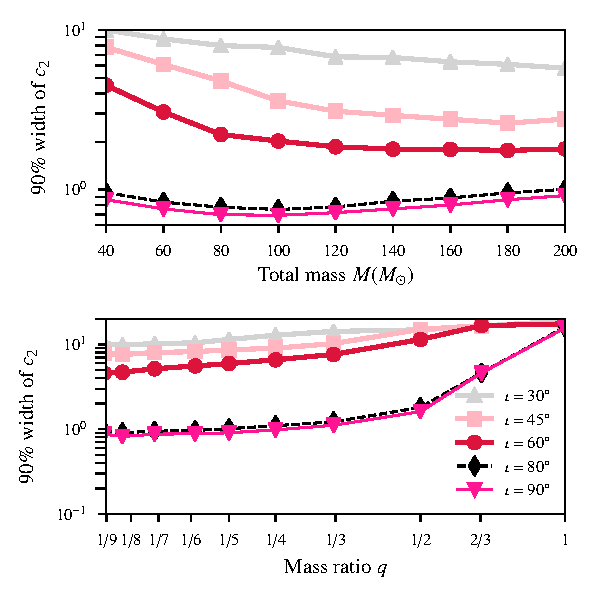
\includegraphics[scale=0.75]{figs/90_percent_bounds_c2.pdf}
		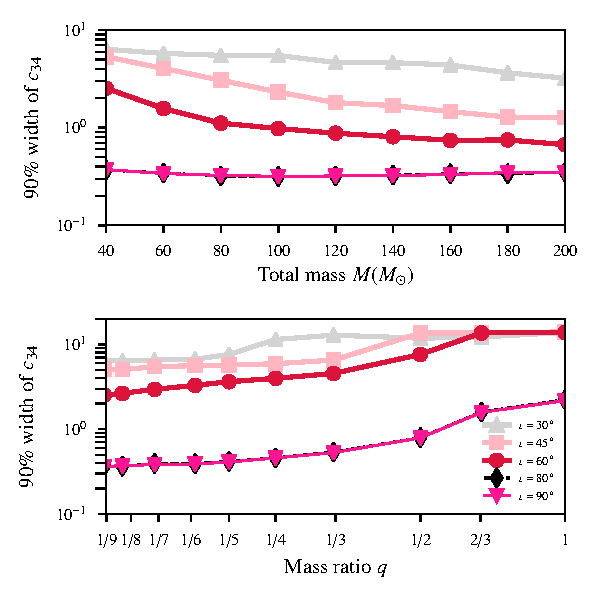
\includegraphics[scale=0.75]{figs/90_percent_bounds_c34.pdf}
	\end{center}
	\caption{Same as Fig.~\ref{fig:constraint_c} except that the posteriors are of the deviation parameters $c_{21}$ (left plots) and  $c_{3344}$ (right plots). \ajith{Pl change the variable names in the plot}}
	\label{fig:constraint_c21_c3344}
\end{figure*}
%%%%%%%%%%%%%%%%%%%%%%%%%%%%%%%%%%%%%%%%%%%%%%%%%%%%%

%%%%%%%%%%%%%%%%%%%%%%%%%%%%%%%%%%%%%%%%%%%%%%%%%%%%%
\begin{figure*}[tbh]
	\centering
	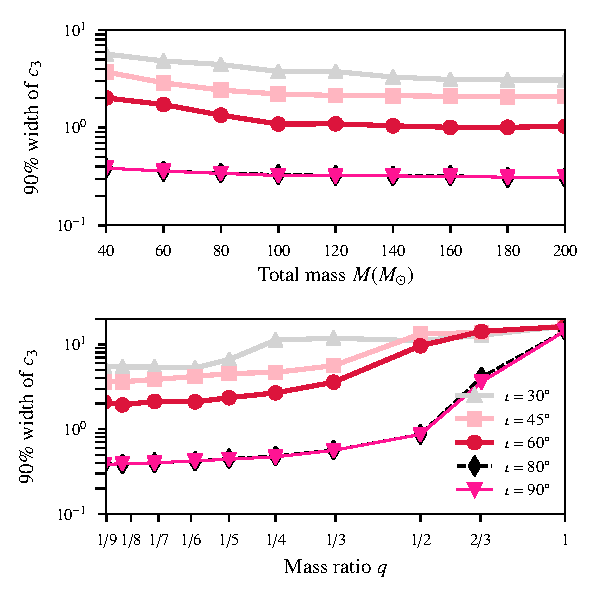
\includegraphics[scale=0.75]{figs/90_percent_bounds_c3.pdf}
	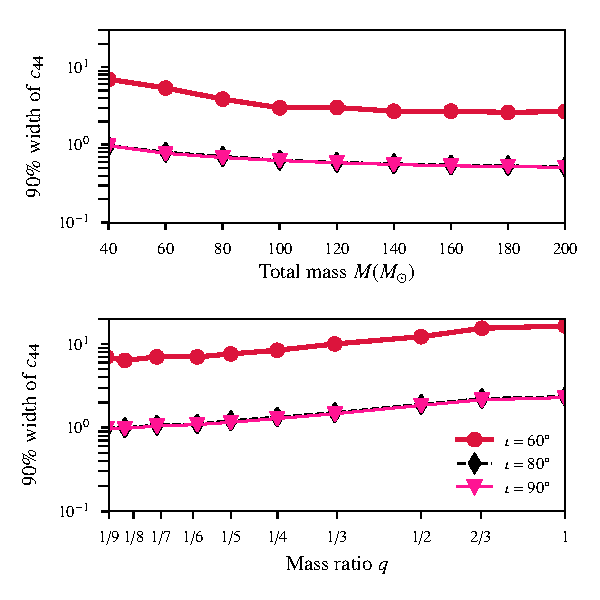
\includegraphics[scale=0.75]{figs/90_percent_bounds_c4.pdf}
	\caption{Same as Fig.~\ref{fig:constraint_c} except that the posteriors are of the deviation parameters $c_{33}$ (left plots) and  $c_{44}$ (right plots).  \ajith{Pl change the variable names in the plot}}
	\label{fig:constraint_c33_c44}
\end{figure*}
%%%%%%%%%%%%%%%%%%%%%%%%%%%%%%%%%%%%%%%%%%%%%%%%%%%

We observe that the constraints on the deviation parameters become narrower for binaries with larger mass ratios and inclination angles. We find that $c$ is, in general, better constrained than $\{c_{21}, c_{3344}\}$ and $\{c_{33}, c_{44}\}$. However, the statistical uncertainties in $c_1$, $\{c_2, c_{34}\}$ and $\{c_3, c_{4}\}$ are modest, reaching only $\sim$ 1 (as opposed to the parameters discussed in Sec.~\ref{sec:formulationA}, which can be constrained to a precision of $\sim 10^{-2}$). The statistical precision of these tests largely depends on the signal-to-noise distribution in the higher modes. These constraints could be significantly improved with third-generation ground based detectors or space based detectors as they will detect hundreds of signals with good SNR and, in turn, enhance the precision of parameter estimation. The low SNR in the higher modes has resulted prior railing for some of the sample chains of $\{c_{21}, c_{3344}\}$ and $\{c_{33}, c_{44}\}$ during MCMC sampling for simulated GR events with binaries having smaller values of total mass, mass ratio and inclination angle
\ajith{Is this true? If yes, this means that we cannot trust these results. Right? If this is the case, we should either rerun these with wider priors, or set the y-axis in Figs 7 and 8 in such a way that these results are beyond the range shown in these plots}. We find that such problems would not arise if the SNR in each of the higher order modes are reasonable high ($\sim 5$). Furthermore, the deviation parameter introduced in our tests, are highly correlated with the luminosity distance $d_L$. This degeneracy introduces some uncertainties in our estimation of bounds.\ajith{Why would it introduce uncertainty in the bounds? Do you mean to say that the statistical uncertainties are larger and the bounds are poorer?}

\section{Simulations with deviations from binary black holes in GR}

\ajith{We can present a more detailed version fo the results presented in Dhanpal et al. I suggest the following figures: 1) comparison of the NSBH/BBH waveforms (perhaps amplitude and frequency of different modes in time domain) 2) 3-detector version of Fig 4 of Dhanpal et al}

%%%%%%%%%%%%%%%%%%%%%%%%%%%%%%%%%%%%%%%%%%%%%%%%%%%%%%%%%%%%%%%%%%%%%%%%%%%%%%%%%%%%%%%%%%
\begin{figure}[htb] 
\begin{center}
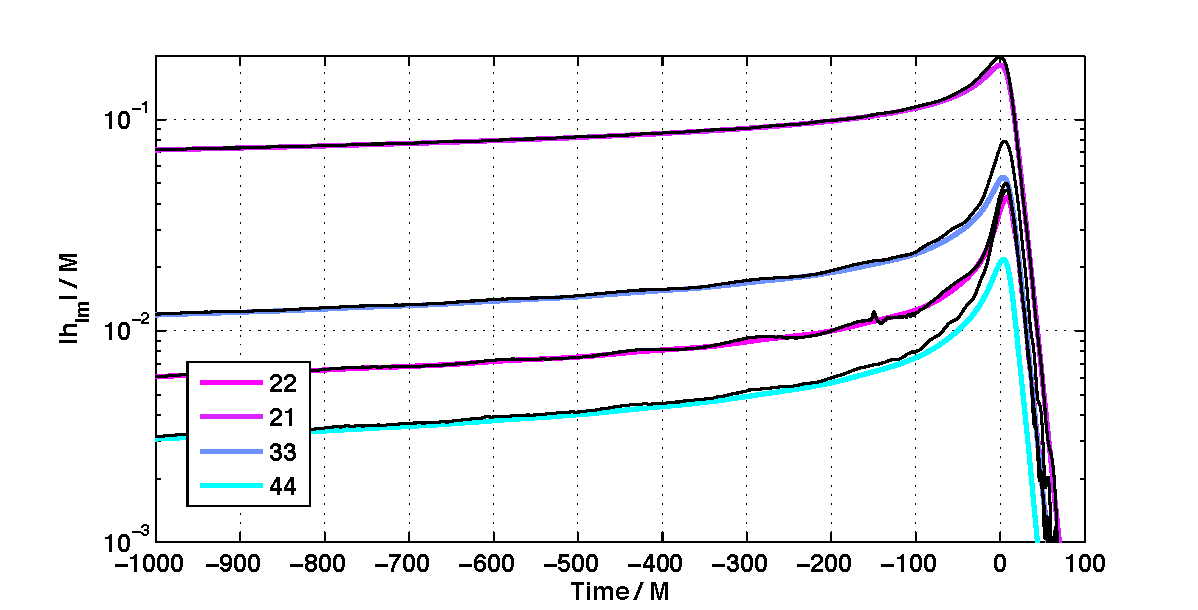
\includegraphics[width=3.4in]{figs/BBH_NSBH_q6_amp.pdf}
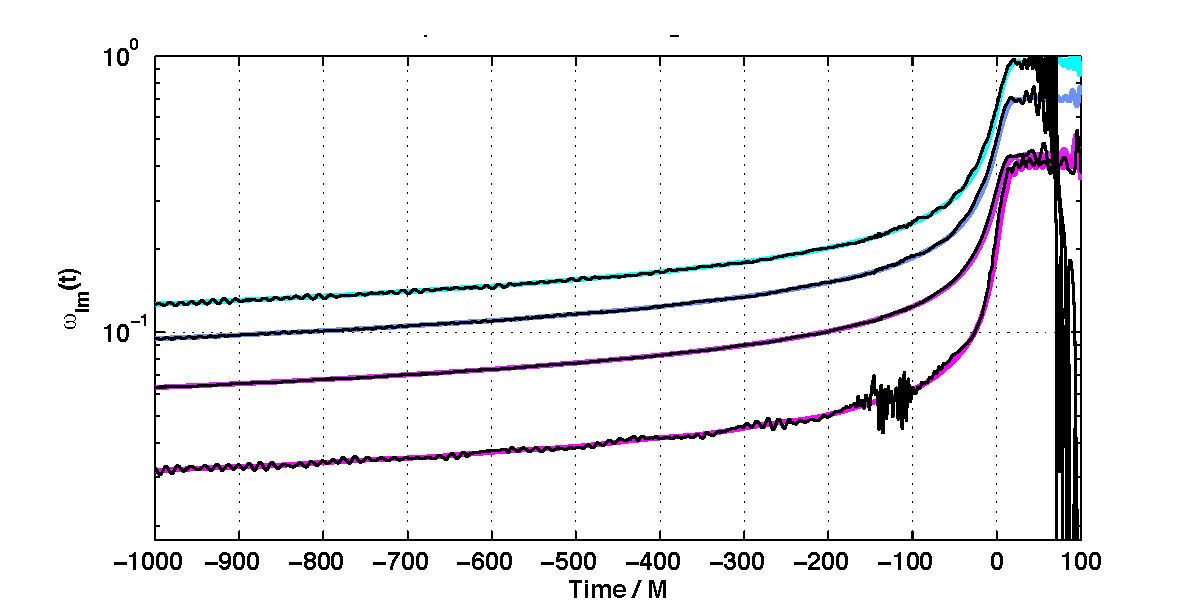
\includegraphics[width=3.4in]{figs/BBH_NSBH_q6_freq.pdf}
\label{fig:bbh_nsbh_waveforms}
\end{center} 
\caption{Time domain amplitude and frequency of different modes of the BBH and rescaled NSBH waveforms.}
\end{figure}
%%%%%%%%%%%%%%%%%%%%%%%%%%%%%%%%%%%%%%%%%%%%%%%%%%%%%%%%%%%%%%%%%%%%%%%%%%%%%%%%%%%%%%%%%%



\section{Waveform systematics}

In all the simulations presented in the previous section, we have assumed that binary black holes have negligible spin angular momenta. While most of the binary black hole events detected by LIGO and Virgo do not appear to have significant spins~\cite{GWTC1}, black holes in binaries, in general, could be spinning. When non-spinning waveform templates are employed to perform the consistency test on GW observations of spinning binaries, the incomplete modeling of the templates can manifest as a deviation from GR. Here we make a first estimate of the effect of neglecting black hole spins in this test by performing the same analysis on simulated spinning binary black hole observations. We simulate spinning binary black hole observations making use of the numerical-relativity surrogate waveform family developed in~\cite{Varma2019} and perform the consistency test using the same non-spinning waveform family~\cite{Mehta} as the base GR waveform over which modifications are applied. 

Figure~\ref{fig:posterior_spin} shows the posteriors in the deviation parameters $\Delta M_c/M_c$ and $\Delta q$ introduced in \eqref{eq:test_1} estimated from simulated binary black hole events with different values of spin. The consistency test is always performed using the non-spinning phenomenological waveform family~\cite{Mehta} as the base GR waveform. The effective spin $\chi_\mathrm{eff} = m_1 \chi_1 + m_2 \chi_2)/(m_1+m_2)$ of the simulated (target) waveforms is shown in the legends. It can be seen that, posteriors estimated from weakly spinning simulated waveforms are largely consistent with the GR values ($\Delta M_c = \Delta q = 0)$ while GW signals with significant spins ($\chi_\mathrm{eff} \gtrsim X)$ produce posteriors that are inconsistent with the GR value. Thus, it is important to model the spin effects in the templates for binaries with considerable spins. 

%%%%%%%%%%%%%%%%%%%%%%%%%%%%%%%%%%%%%%%%%%%%%%%%%%%%%%%%%%%%%%%%%%%%%%%%%%%%%%%%%%%%%%%%%%
\begin{figure}[htb] 
\begin{center}
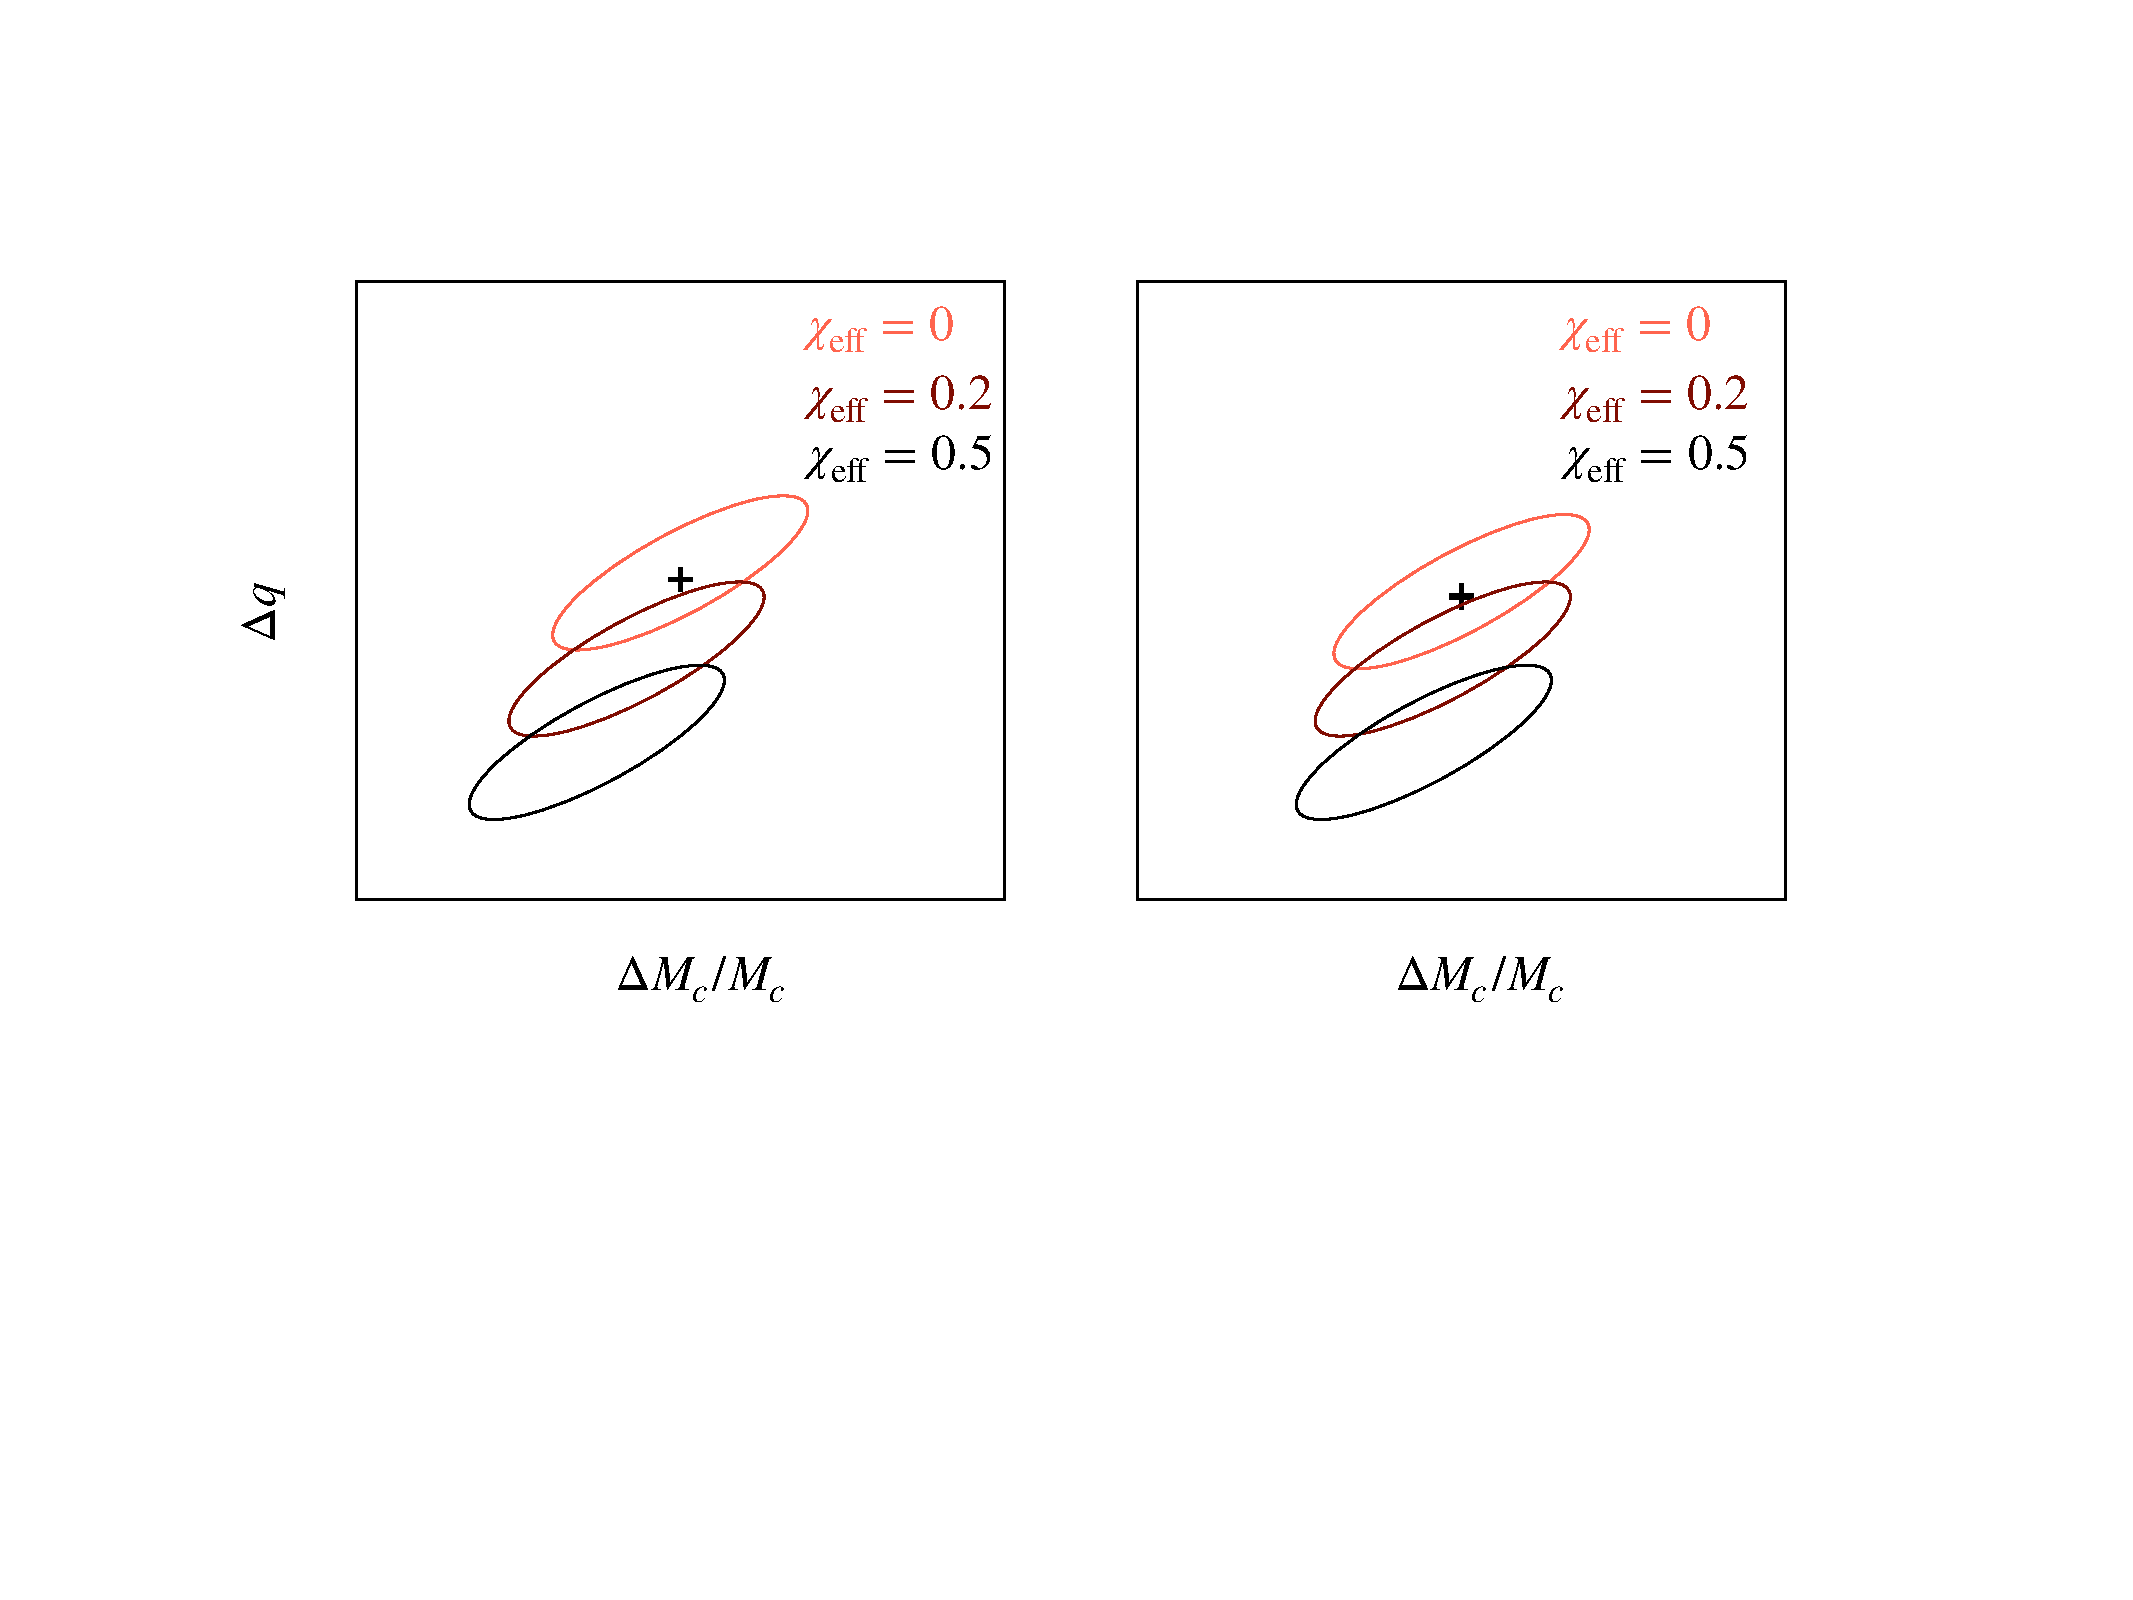
\includegraphics[width=3.4in]{figs/cartoon_plot.pdf}
\label{fig:posterior_spin}
\caption{Fake posteriors from spinning injections. Replace this with right plots}
\end{center} 
\end{figure}
%%%%%%%%%%%%%%%%%%%%%%%%%%%%%%%%%%%%%%%%%%%%%%%%%%%%%%%%%%%%%%%%%%%%%%%%%%%%%%%%%%%%%%%%%%

\section{Discussions \& Conclusion}
In this paper, we have proposed a set of tests of the ``no-hair'' nature of binary black holes in GR based on a consistency test of the multipolar structure of the gravitational radiation. These tests are analogous to the tests of ``no-hair'' theorem for stationary black holes based on the consistency of different quasi-normal modes of a perturbed black hole~\cite{xx}. We proposed two formulations of this test, that introduce extra deviation parameters that goveren the amplitude and phase evolution of different spherical harmonic modes of the radiation, as well as ones affecting the amplitudes of different modes. Posterior distributions of these deviation parametrs can be estimated using a Bayesian framework. 

The first formulation is inspired by the fact that different modes of radiation from the BBH should be uniquely described only by the same values of intrinsic parameters (chirp mass and mass ratio), and hence these parameters estimated from different modes should be consistent to each other. We first revisited this formulation, originally presented in~\cite{dhanpal2018}. We presented the results expected from 3-detector observations of binary black holes using the Advanced LIGO-Virgo detectors. Results from our simulations suggest that upcoming observations using Advanced LIGO and Virgo will be able to put precise constraints on the deviation parameters. Indeed, this test requires appreciable SNR in the higher order modes of the observed GW signal, which is expected only for small fraction (a few percents~\cite{Dhanpal}) of detectable binary black hole events. However, given that LIGO-Virgo would observed hundreds of binary black hole mergers in coming years, we expect a reasonable number of such events to be observed. We also demonstrate that, if the observed signal is not produced by a binary black hole system in GR, the test is able to identify this, provided that the SNR is high enough. 

In the second formulation, we check for the consistency between the amplitudes of different modes. In order to do so, we introduce a set of extra deviation parameters in the amplitudes for the higher modes. We see that these deviation parameters can be constrained only with modest precision in Advanced LIGO-Virgo. However, the precision of such a test is expected to increase manifold with the next generation of detectors (e.g. with Einstein Telescope or LISA). 

We also present a preliminary investigation of the effect of neglecting the effect of black hole spin in the analysis and find that if the binary has significant effective spin, neglecting spin effects can produce a bias in the estimated posteriors. This can mock a GR violation. 

\ajith{Need to make some concluding remarks}


\newpage
\bibliography{TestGR.bib}

\end{document}
